\section{Risk Assessment}
\label{sec:risk-assessment}

\subsection{Rating scheme}

The risk assessment follows the concept phase of ISO/SAE~21434~\cite{iso21434}
and reuses the rating template already applied by the group in an earlier TARA,
so that the results remain comparable. Each threat receives an impact rating in
the four categories of the standard, namely safety, financial, operational and
privacy. The four ratings are combined into a single impact value with the
weights of Table~\ref{tab:scales}, which give the safety category a dominant
role. Attack feasibility is derived from the attack vector of the affected
element, an approach permitted by the standard when a full attack potential
rating is not yet available. The risk score is one plus the product of impact and
feasibility, and is mapped to a risk value on a four-level scale. Risks rated Low are retained;
all others are treated by risk reduction.

\begin{table}[htbp]
\centering
\caption{Rating scheme used for the risk assessment}
\label{tab:scales}
\footnotesize
\begin{tabularx}{\columnwidth}{lX}
\toprule
\textbf{Parameter} & \textbf{Definition} \\
\midrule
Impact rating per category & Severe 10, Major 7, Moderate 4, Negligible 1 \\
Category weights & Safety 5, Operational 1, Financial 0.5, Privacy 0.25 \\
Impact value $I$ & $(5S + 1O + 0.5F + 0.25P)/4$ \\
Severity level & Severe $\geq 8.3$, Major $\geq 5.1$, Moderate $\geq 2.5$, Negligible $\geq 1$ \\
Feasibility value $F$ & Network 10, Adjacent 7, Local 4, Physical 1 \\
Risk score $R$ & $1 + I \times F$ \\
Risk value & Critical $\geq 100$, High $\geq 49$, Medium $\geq 16$, Low $\geq 1$ \\
Risk treatment & Reduction for Critical, High and Medium; retention for Low \\
\bottomrule
\end{tabularx}
\end{table}

\subsection{Scope of the assessment}

The rating scheme was applied to two sets. The first is the complete output of
medini analyze for the architecture model: 225 threats, of which 72 concern the
12 components and cover all six STRIDE categories, 102 concern the 34 component
ports and 51 the 17 connections. For ports and connections the tool generates
only tampering, information disclosure and denial of service. Medini enumerates
each threat as a pair of model element and STRIDE category without a damage
scenario or attack path, so the ratings of this set apply to the pair as a
whole.

The second set contains the 170 concrete threat scenarios produced by the LLM
configurations, rated outside the tool with the same template. Each scenario
was assigned to an architecture element and matched with medini on element and
STRIDE category, as described in Section~\ref{sec:comparison}; asset labels
that combine several elements were assigned to the first element named. 151
scenarios fall on a pair that medini also enumerates and describe a specific
way in which that threat can be realised. The remaining 19 lie outside the
enumeration of the tool: 12 concern assets that have no element in the model,
namely the AI models, prompts and agent configuration and the end-to-end data
flow, and 7 are spoofing or repudiation threats on communication links,
categories that medini does not generate for connections. The complete
worksheets, with the medini identifiers, the scenario descriptions and the
individual ratings, are provided as supplementary material.

\subsection{Results for the medini threats}

Table~\ref{tab:risk_medini} summarises the 225 threats by architecture element.
70 are Critical, 69 High, 72 Medium and 14 Low, with an average risk score of
61.8. The Critical band holds only two distinct values. The 27 threats rated
104.7 concern elements reached over an adjacent link with severe impact: the
DENM encoder, the RSU, the OBU, the central ITS-S and the link between encoder
and RSU. The 43 threats rated 104.1 are reachable over the network, with the
safety impact rated major: the edge detector, the three agents, the cloud MLLM
and the cellular and sidelink connections. Elements that require local access,
namely the cameras, the vehicle computer, the driver HMI and the in-vehicle
links, do not exceed High (60.3). The highest value below the Critical band,
83.7, belongs to denial of service at the warning output of the OBU.

\begin{table}[htbp]
\centering
\caption{Risk assessment of the medini threats by architecture element. For
components, $n$ counts the threats on the component and its ports; for
connections, the threats on all links of the group. Vector: L local,
A adjacent, N network.}
\label{tab:risk_medini}
\footnotesize
\setlength{\tabcolsep}{3.2pt}
\begin{tabularx}{\columnwidth}{Xcrrrrrr}
\toprule
\textbf{Element (step)} & \textbf{Vec.} & \textbf{$n$} & \textbf{C} & \textbf{H} & \textbf{M} & \textbf{L} & \textbf{$R_{\max}$} \\
\midrule
\multicolumn{8}{l}{\textit{Roadside station}} \\
\quad Cameras (1) & L & 9 & -- & 4 & 2 & 3 & 60.3 \\
\quad Edge detector (2) & L/N & 12 & 4 & 3 & 4 & 1 & 104.1 \\
\quad Agent 1, situation (3) & N & 18 & 7 & 5 & 6 & -- & 104.1 \\
\quad Agent 2, distance (5) & N & 12 & 5 & 3 & 4 & -- & 104.1 \\
\quad Agent 3, message (6) & N & 18 & 7 & 5 & 6 & -- & 104.1 \\
\quad DENM encoder (8) & A & 12 & 5 & 3 & 4 & -- & 104.7 \\
\quad RSU (9) & A & 18 & 7 & 5 & 6 & -- & 104.7 \\
\addlinespace[2pt]
\multicolumn{8}{l}{\textit{Cloud and back end}} \\
\quad Cloud MLLM (4, 7) & N & 18 & 7 & 5 & 6 & -- & 104.1 \\
\quad Central ITS-S (10) & A & 18 & 7 & 5 & 6 & -- & 104.7 \\
\addlinespace[2pt]
\multicolumn{8}{l}{\textit{Vehicle}} \\
\quad OBU (11) & A & 18 & 7 & 5 & 6 & -- & 104.7 \\
\quad Vehicle computer (12) & L & 12 & -- & 5 & 3 & 4 & 60.3 \\
\quad Driver HMI (13) & L & 9 & -- & 4 & 2 & 3 & 60.3 \\
\addlinespace[2pt]
\multicolumn{8}{l}{\textit{Connections}} \\
\quad Intra-station (6 links) & L/A/N & 18 & 5 & 6 & 6 & 1 & 104.7 \\
\quad 5G Uu (8 links) & N & 24 & 8 & 8 & 8 & -- & 104.1 \\
\quad PC5 sidelink (1 link) & N & 3 & 1 & 1 & 1 & -- & 104.1 \\
\quad In-vehicle (2 links) & L & 6 & -- & 2 & 2 & 2 & 60.3 \\
\midrule
Total & & 225 & 70 & 69 & 72 & 14 & 104.7 \\
\bottomrule
\end{tabularx}
\end{table}

Fig.~\ref{fig:risk_heatmap} breaks the ratings down by STRIDE category. The
category bounds the risk value and the zone of the element places it within
those bounds: tampering, spoofing and elevation of privilege are Critical or
High, denial of service is High or Medium, and information disclosure and
repudiation are Medium or Low. The figure also shows how the
modelling granularity shapes the list. Every data flow is represented by an
output port, an input port and a connection, so the same threat appears up to
three times along one flow with identical ratings; tampering of the detection
list, for example, is listed as T023, T026 and T035. Port and connection
threats make up 153 of the 225 entries, which is why tampering, information
disclosure and denial of service account for 84\% of the set.

\begin{figure}[htbp]
    \centering
    \includegraphics[width=\columnwidth]{fig_risk_heatmap.png}
    \caption{Highest risk score of the medini threats per architecture element
    and STRIDE category. Small numbers give the count of threats in the cell
    when it exceeds one; n/g marks categories that medini does not generate for
    connections. The last column gives the attack vectors in the row.}
    \label{fig:risk_heatmap}
\end{figure}

\subsection{Results for the LLM scenarios}

Of the 170 scenarios, 58 are Critical, 53 High, 46 Medium and 13 Low, with an
average risk score of 64.2. Table~\ref{tab:risk_llm} breaks the set down by
model and by relation to the medini enumeration. The category bounds found in
the medini set hold here without exception: all 58 Critical scenarios are
spoofing, tampering or elevation of privilege, and no information disclosure
or repudiation scenario exceeds Medium.

% NOTE: the per-model rows reflect the current worksheet. Check that the
% DeepSeek and Copilot rows (and the second Claude configuration) are complete.
\begin{table}[htbp]
\centering
\caption{Risk assessment of the LLM scenarios by model and by relation to the
medini enumeration. Elem.\ counts the architecture elements addressed; $\bar{R}$
is the average risk score.}
\label{tab:risk_llm}
\footnotesize
\setlength{\tabcolsep}{3.2pt}
\begin{tabularx}{\columnwidth}{Xrrrrrrr}
\toprule
\textbf{Group} & \textbf{$n$} & \textbf{Elem.} & \textbf{C} & \textbf{H} & \textbf{M} & \textbf{L} & \textbf{$\bar{R}$} \\
\midrule
\multicolumn{8}{l}{\textit{By model}} \\
\quad ChatGPT & 90 & 17 & 32 & 25 & 26 & 7 & 63.9 \\
\quad Claude & 57 & 14 & 20 & 18 & 15 & 4 & 65.6 \\
\quad Gemini & 18 & 7 & 6 & 7 & 4 & 1 & 65.7 \\
\quad DeepSeek & 4 & 1 & -- & 2 & 1 & 1 & 45.1 \\
\quad Copilot & 1 & 1 & -- & 1 & -- & -- & 60.3 \\
\addlinespace[2pt]
\multicolumn{8}{l}{\textit{By relation to the medini enumeration}} \\
\quad Pair enumerated by medini & 151 & 15 & 47 & 51 & 40 & 13 & 62.5 \\
\quad Category not generated for links & 7 & 3 & 5 & -- & 2 & -- & 83.9 \\
\quad Asset without model element & 12 & 2 & 6 & 2 & 4 & -- & 73.8 \\
\midrule
Total & 170 & 17 & 58 & 53 & 46 & 13 & 64.2 \\
\bottomrule
\end{tabularx}
\end{table}

The 19 scenarios outside the enumeration of the tool are rated markedly higher
than the rest. Eleven of them are Critical (58\%), against 47 of the 151
scenarios on enumerated pairs (31\%), and their average risk scores of 83.9 on
links and 73.8 on assets without a model element exceed the 62.5 of the
enumerated pairs. Table~\ref{tab:risk_llm_only} lists them. They include prompt
injection that gives an agent access to tools and the operating system,
manipulation of model files, prompts and agent policies, use of a compromised
low-trust component as a pivot towards the AI, PKI and V2X assets, and
spoofing on the PC5 and Uu links.

% NOTE: model attribution in this table depends on the completeness of the
% worksheet (see note above).
\begin{table}[htbp]
\centering
\caption{LLM scenarios outside the medini enumeration}
\label{tab:risk_llm_only}
\footnotesize
\setlength{\tabcolsep}{3.5pt}
\begin{tabularx}{\columnwidth}{c>{\raggedright\arraybackslash}Xrl}
\toprule
\textbf{ST.} & \textbf{Scenario} & \textbf{$R$} & \textbf{Model} \\
\midrule
\multicolumn{4}{l}{\textit{AI models, prompts and agent configuration}} \\
S & Unapproved model presented as an approved component & 104.1 & ChatGPT \\
T & Model files, prompts or agent policies altered & 104.1 & ChatGPT \\
R & No provenance of model version and prompt & 32.9 & ChatGPT \\
I & Prompts and model outputs exposed through debug interfaces & 23.5 & ChatGPT \\
D & Crafted inputs exceed the real-time inference capacity & 74.1 & ChatGPT \\
E & Prompt injection grants access to tools, files or the OS & 104.1 & ChatGPT \\
\addlinespace[2pt]
\multicolumn{4}{l}{\textit{End-to-end data flow}} \\
S & False accident event accepted as a trusted detection & 104.1 & ChatGPT \\
T & Event data altered between pipeline stages & 104.1 & ChatGPT \\
R & No correlation identifiers to reconstruct an event & 32.9 & ChatGPT \\
I & Sensitive data exposed at intermediate stages & 23.5 & ChatGPT \\
D & Disruption of any stage suppresses a valid warning & 74.1 & ChatGPT \\
E & Pivot from a low-trust component to AI, PKI or V2X assets & 104.1 & ChatGPT \\
\addlinespace[2pt]
\multicolumn{4}{l}{\textit{Certificates and event reports (0)}} \\
S & Forged certificates or event reports accepted as genuine & 104.1 & ChatGPT \\
S & Stolen certificate authenticates a rogue RSU or OBU & 104.1 & Claude \\
R & Missing signatures and timestamps prevent attribution & 32.9 & ChatGPT \\
R & Sender denies a fraudulent event report & 32.9 & Claude \\
\addlinespace[2pt]
\multicolumn{4}{l}{\textit{5G Uu links}} \\
S & Endpoint impersonates the cloud or roadside service & 104.1 & ChatGPT \\
\addlinespace[2pt]
\multicolumn{4}{l}{\textit{PC5 sidelink (9$\rightarrow$11)}} \\
S & Forged vehicle or RSU safety messages & 104.7 & ChatGPT \\
S & GNSS spoofing combined with message replay & 104.7 & Claude \\
\bottomrule
\end{tabularx}
\end{table}

\subsection{Comparison of the two sets}

At the level of the risk distribution the two sets are close
(Fig.~\ref{fig:risk_distribution}): 31.1\% of the medini threats and 34.1\% of
the LLM scenarios are Critical, 30.7\% and 31.2\% High, 32.0\% and 27.1\%
Medium, and 6.2\% and 7.6\% Low. The similarity arises for different reasons,
as Fig.~\ref{fig:risk_stride} shows. The medini list is dominated by
tampering, information disclosure and denial of service, the categories
repeated on ports and connections; tampering raises the Critical share and
information disclosure the Medium share by about the same amount. The LLM
scenarios are spread more evenly across the categories and give spoofing and
elevation of privilege 31\% of the set, against 11\% in medini. A comparison
at the level of the distribution therefore hides a difference in content.

\begin{figure}[htbp]
    \centering
    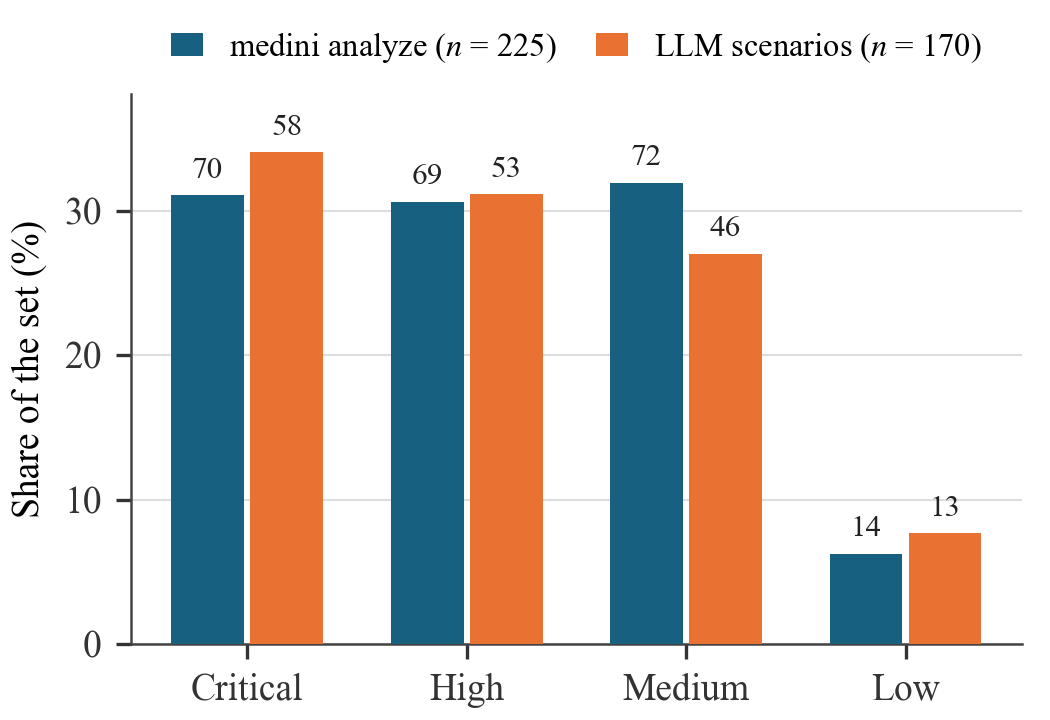
\includegraphics[width=\columnwidth]{fig_risk_distribution.png}
    \caption{Distribution of risk values in the medini threats and the LLM
    scenarios, as a share of each set. Labels give the absolute counts.}
    \label{fig:risk_distribution}
\end{figure}

\begin{figure}[htbp]
    \centering
    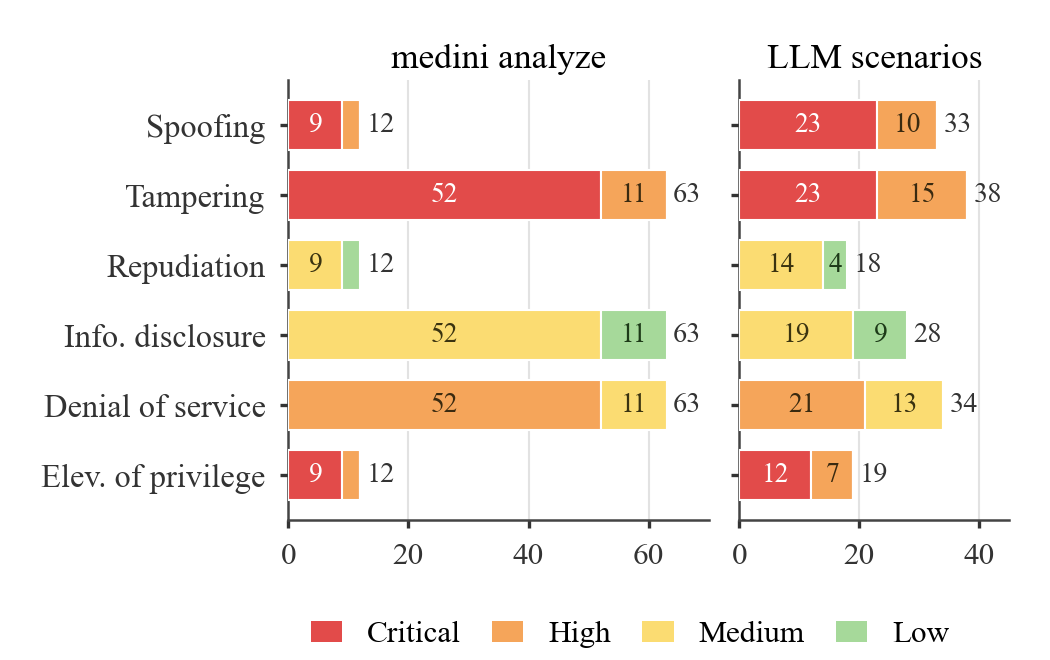
\includegraphics[width=\columnwidth]{fig_risk_stride.png}
    \caption{Number of medini threats and LLM scenarios per STRIDE category,
    by risk value.}
    \label{fig:risk_stride}
\end{figure}

The risk matrices of Fig.~\ref{fig:risk_matrix} confirm that both sets were
rated on the same grid. They occupy the same cells: no threat is rated as
requiring physical access, and a major impact never occurs together with local
access. Some cells mix risk values because the Severe band spans impact values
from 8.3 to 16.9, so a severe threat with local access is High or Medium, and
one with adjacent access Critical or High, depending on its exact impact
value. The matrices also show the weight of
reachability. Threats with negligible impact that can be reached over an
adjacent or network link are rated Medium, 37 in the medini set and 12 among
the LLM scenarios, while threats with moderate impact that require local
access are rated Low.

\begin{figure*}[htbp]
    \centering
    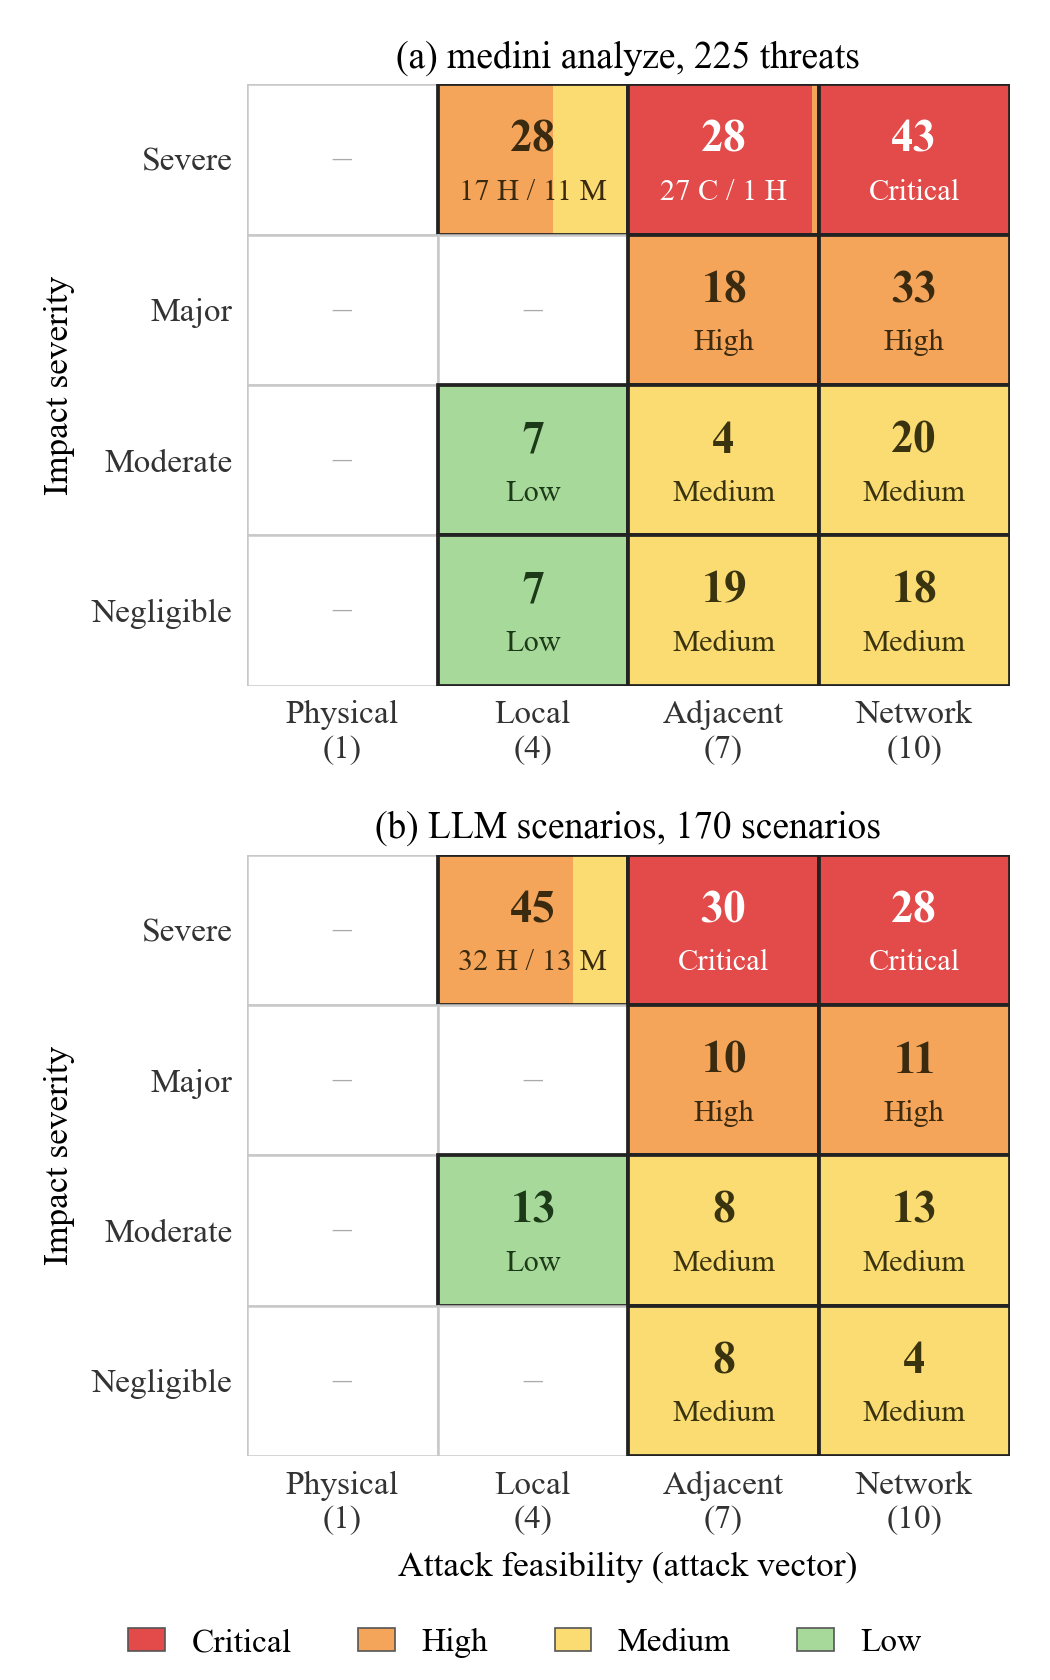
\includegraphics[width=0.92\textwidth]{fig_risk_matrix.png}
    \caption{Risk matrices of (a) the medini threats and (b) the LLM scenarios.
    Each cell gives the number of threats and their risk value; cells with
    mixed values are split in proportion to the counts (C Critical, H High,
    M Medium). Dashes mark combinations that do not occur.}
    \label{fig:risk_matrix}
\end{figure*}

\subsection{Observations}

Five observations follow from the tables and figures.

First, the rating is driven by the STRIDE category rather than by the
content of a threat. All 128 Critical ratings in the two sets are spoofing,
tampering or elevation of privilege: these categories received the highest
safety ratings, denial of service intermediate ones, and information disclosure
and repudiation a negligible safety impact throughout. With a safety weight of 5 and a
privacy weight of 0.25, a confidentiality breach with severe privacy impact and
negligible safety impact reaches an impact value of 2.6 (Moderate), so the
exposure of camera images that show faces and licence plates is rated Low or
Medium, even though it may have legal consequences under data protection law.

Second, the scheme cannot rank threats within the Critical band. The 225
medini threats take only 15 distinct risk scores and the 170 LLM scenarios 14.
The 70 Critical medini threats share two values that differ by 0.6, and that
difference reflects the safety impact assigned to a zone, major for the
network-reached AI stages and severe for the V2X chain, rather than a
difference between individual threats. Prioritisation inside the band needs
feasibility and impact rated per threat.

Third, attacks that act through the physical environment of the camera are
not represented by the attack vector taxonomy. Staged scenes, adversarial
patches and blinding with a laser require no access to any system, yet they
inherit the local vector of the camera zone: the spoofing and tampering
variants are rated High (60.3), exactly like attacks on the network interface
of the camera, and blinding as a denial of service is rated Medium (48.3). The
rating neither reflects the low effort these attacks require nor separates them
from attacks that need access to the device, which argues for a full attack
potential rating in the next iteration.

Fourth, the scenarios outside the enumeration of the tool are the most severe
part of the LLM set. The architecture model has no element for the AI models,
prompts and agent configuration or for the end-to-end data flow, and medini
generates no spoofing or repudiation threats for connections. The 19 scenarios
in these gaps include 11 Critical ones, among them prompt injection with access
to tools and the operating system and pivoting from a low-trust component. A
tool-based analysis would raise them only after the model is extended with
AI-specific assets.

Fifth, the 27 Low risks, 14 medini threats and 13 LLM scenarios, are retained;
all other risks are treated by reduction.
% TODO: the new worksheets contain no measures column; check that the control
% groups below still match the proposed controls.
The proposed controls fall into five groups: message signing with certificate
verification and plausibility checks in the vehicle; protection of the
transport paths through mutual authentication, certificate pinning and
authenticated internal links; platform hardening with secure boot, signed
software and signed model files; records that link every generated message to
the input frame, the prompt version and the model response; and
privacy-preserving pre-processing of the images before they leave the roadside
station.

\subsection{Limitations}

The impact ratings are qualitative expert judgements of the authors, derived
for a motorway deployment; a different operational context would change the
safety and operational categories. The ratings were assigned per STRIDE
category and architectural zone with few element-specific adjustments, so
threats of the same category and zone share a score, which limits the
resolution of the ranking. Attack feasibility is rated from the attack vector
of the element alone, which ignores the elapsed time, expertise and equipment
that the full attack potential approach of ISO/SAE~21434 considers. Finally,
the LLM scenarios were rated outside the tool and assigned to architecture
elements by hand; scenarios that address several elements were counted under
the first element named.
